\documentclass[12pt,a4paper]{article}
\usepackage[T1]{fontenc}
\usepackage[utf8]{inputenc}
\usepackage[italian]{babel}
\usepackage{lmodern}
\usepackage{graphicx}
\usepackage{minted}
\usepackage{hyperref}
\usepackage{dirtree}

\setlength{\parindent}{2em}
\setlength{\parskip}{1em}

\setminted[python]{frame=lines,framesep=1em}

\newcommand{\mrcnn}{Mask-R\_CNN}

\begin{document}

\title{Riconoscimento Documenti}
\author{Simone Cimarelli \and Vittorio Mignini \and Luca Moroni}
\date{9 luglio 2020}

\maketitle

\begin{abstract}
    Si descrive l'implementazione di un applicativo, che permette il
    riconoscimento in tempo reale di un set di tipologie di documenti a
    priori definite.
\end{abstract}

\section{Obbiettivi}

Implementare un applicativo che tramite l'utilizzo di un dispositivo di
input video sia in grado di riconoscere e di identificare un insieme di
documenti a priori definiti e di riconoscere delle porzioni di testo
presenti nel documento precedentemente identificato.

\section{Analisi dei Requisiti}
\subsection{Analisi Requisiti Utente}

\begin{itemize}
    \item Ottenere un elenco dei documenti visibili all'interno di
        un'immagine e le componenti testuali specifiche in esso
        riconoscibili.
    \item Avere la possibilità di definire la natura dei documenti
        oggetto del riconoscimento e delle informazioni testuali
        rilevanti in essi contenute.
    \item Mettere a disposizione un interfaccia grafica semplice e
        minimale per l'acquisizione di video e immagini
\end{itemize}

\subsection{Analisi Requisiti Sistema}

\begin{itemize}
    \item Implementare delle tecnologie per l'object detection e ocr
        allo stato dell'arte per erogare in modo efficiente il servizio
        richiesto dal committente.
    \item Fornire strumenti che mettono a disposizione la possibilita di
        rendere scalabile il numero e la tipologia di documenti
        riconoscibili dall'applicativo
    \item L'applicativo finale \textit{dovrebbe} essere portabile e non
        strettamente dipendente da una particolare architettura
\end{itemize}

\subsection{Glossario e Dominio applicativo}

Il prodotto risponde all'esigenza di individuare la tipologia ed
eseguire il parsing dei prinicipali dati testuali esposti in vari
documenti di riconoscimento, tramite webcam.
I domini applicativi di tale sistema e le problematiche ad essi connesse
sono sono quelli dell'ambito della computer vision e dell'OCR.
L'utente finale avrà a disposizione un'interfaccia grafica attraverso la
quale, in modo intuitivo ed efficiente, potrà avere accesso al servizio
erogato.

\begin{description}
    \item[Computer Vision] Insieme di metodologie algoritmiche e
        matematiche che hanno come obiettivo quello di acquisire delle
        conoscenze ad alto livello partendo da immagini o video. Nel
        nostro caso capire se e dove nelle immagini passate
        all'applicativo è presente un documento del tipo prestabilito.
    \item[Object Detection] Tecnologia relativa all'ambito della
        computer vision, che propone una soluzione algoritmica per il
        riconoscimento di istanze riguardanti oggetti di classi
        predefinite in immagini digitali e video.
    \item[OCR] Optical Character Recognition, metodologie software per
        il riconoscimento di caratteri contenuti in un documento e
        trascrizione di tali simboli in caratteri equivalenti.
\end{description}

\subsection{Modellazione Concettuale del Sistema}

Il compito di interagire con l'utente finale sarà a carico di una
componente di interfaccia grafica ``frontend'' che si occuperà
dell'accesso alla videocamera e mostrerà uno storico dei documenti
riconosciuti e in corso di riconoscimento in tempo reale, mentre
delegherà il compito di applicare e interpretare i risultati delle
primitive di riconoscimento e OCR a una componente ``buisiness logic''
configurabile dal committente potendo scegliere il tipo di documenti da
riconoscere e le carateristiche testuali da ricercare.

\section{Architettura del Sistema}

In fase di revisione dei requisiti, si sono andati a definire quelli che sono i requisiti
funzionali del nostro applicativo tramite l'utilizzo del diagramma di
caso d'uso.

\subsection{Diagramma di caso d'uso per il funzionamento di
riconoscimento}

Tale diagramma necessario nella prima fase di progettazione ha messo sul
tavolo quella che è a grandi linee la logica applicativa del nostro
sistema per quanto riguarda il funzionamento "effettua riconoscimento", si noti la ripartizione e la differenziazione di quattro principali
casi d'uso, ovvero il riconoscimento sul quale si interfaccia
direttamente il nostro attore principale, dove quest'ultimo si posiziona davanti alla telecamera con in mano un documento. Il caso d'uso riconoscimento
implementerà il caso d'uso riconosci documento, che definisce la collocazione di
utilizzo di una possibile funzionalità di object detection, quest'utlimo
includera poi il caso d'uso effettua ocr.
Infine il quarto caso d'uso visualizza documenti, con il quale l'attore principale si interfaccerà direttamente e tramite il quale sarà in grado di
visualizzare i documenti riconosciuti fino a quel momento.

\begin{figure}[H]
    \caption{Diagramma di Caso d'Uso}
    \centering
    \includegraphics[width=\textwidth,height=\textheight,keepaspectratio]{uml_use_case.pdf}
\end{figure}

\subsection{Scelte architetturali}

Nella progettazione architetturale di tale applicativo, si è optato per
l'utilizzo di librerie testate e rappresentanti lo stato dell'arte,
inerentemente all'ambito applicativo sopracitato.\\
Per quanto riguarda l'object detection, abbiamo selezionato la libreria
\textbf{\mrcnn} una libreria che oltre a effettuare object detection mette a
disposizione anche segmentazione di immagini, una feature aggiuntiva che
oltre a ritornare un rettangolo contenente un oggetto di una determinata
classe nell'immagine ne ritorna anche la regione di pixel che lo
rappresenta, tale feature comunque non è utilizzata nel nostro sistema,
ma è tornata utile in fase di training in quanto possiamo allenare la
nostra rete direttamente tramite i segmenti di documenti, evitando la
presenza dei polpastrelli che in alcuni casi possono portare la nostra
rete fuori rotta.\\
Invece per effettuare l'ocr abbiamo optato per la libreria tesseract,
resa disponibile in python tramite una libreria wrapper chiamata
pytesseract.

Le librerie appena citate hanno portato alla necessità di importarne
altre tra cui, tensorflow$=$1.x, flask$=$2.0.8 sulle quali si basa
\mrcnn, opencv per la gestione e la codifica di immagini.

Per la gestione delle dipendenze in fase di sviluppo abbiamo utilizzato
due strumenti propri dell'ambiente python, pipenv che mette a
disposizione un ambiente virtuale contenente determinate librerie in
modo asettico rispetto a quelle di sistema e che rende ripetibile su
altre macchine la configurazione da noi utilizzata con semplici
passaggi. pyenv che invece mette a disposizione delle versioni di python
proprie in modo da non andare a modificare quella di sistema nel caso
sia necessaria un versione non corrispondente con quella di sistema, ad
esempio tensorflow$=$1.x è utilizzabile solamente con versioni di
python$\leq$3.7.x con pyenv tale requisito puo essere soddisfatto su
qualsiasi macchina.

Data la complessita computazionale delle operazioni messe a disposizione
dalle librerie \mrcnn\ e pytesseract, si è optato per effettuare il
processing di singoli frame intercorsi da quanti temporali variabili a
seconda del precedente riconoscimento, e non di uno stream video
continuo, questo perchè non sarebbe garantita una fluidità
nell'erogazione del servizio su gran parte parte delle macchine server
sulle quali questa web app puo essere esposta.

\subsection{Accenni strutturali di \mrcnn}

Il funzionamento della rete \mrcnn\ consiste in due fasi. Nella prima
fase la rete ritorna delle regioni le quali dovrebbero rappresentare
oggetti presenti sull'immagine di input. La seconda fase invece,
effettua un inferenza sulla classe dell'oggetto, rifinisce il bounding
box e genera la maschera, a livello di pixel, basandosi sull'output
della prima fase. Entrambe le fasi sono connesse alla struttura
backbone.

\begin{figure}[H]
    \caption{Struttura \mrcnn}
    \centering
    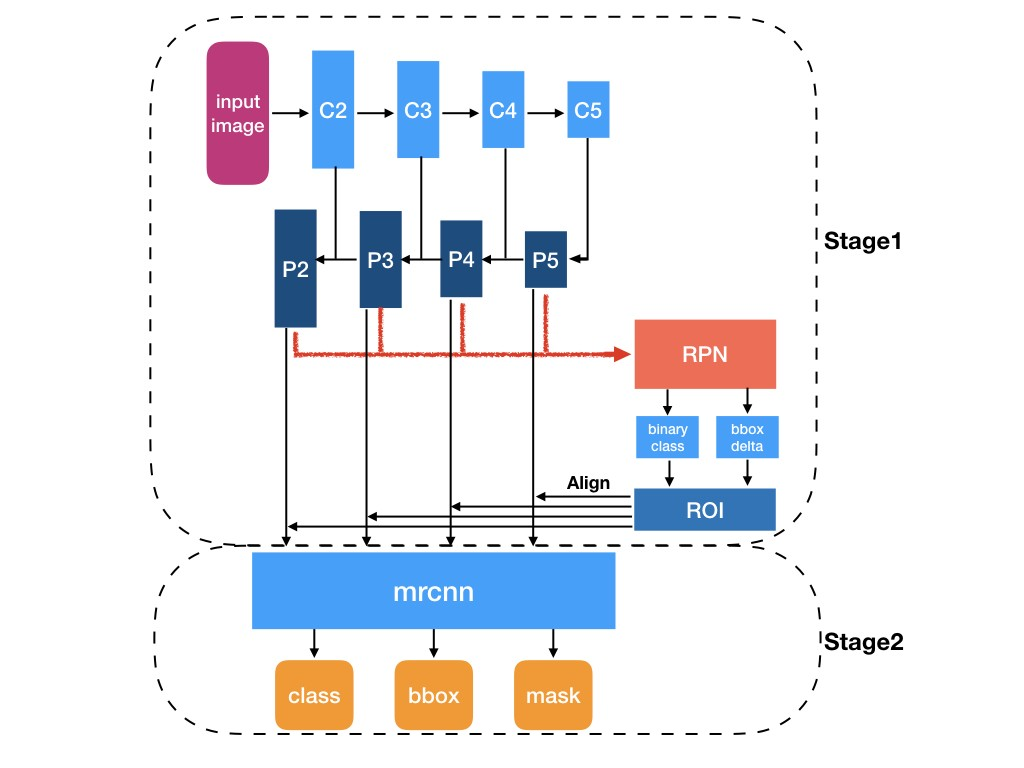
\includegraphics[width=\textwidth,height=\textheight,keepaspectratio]{mask_description.jpeg}
\end{figure}

\subsection{Training}

Avendo deciso che la bussiness logic del nostro sistema si basa su una rete
neurale per la computer vision implementata tramite la libreria \mrcnn, cioè una
rete neurale molto complessa sulla quale facciamo transfer learning, ovvero
alleniamo solamente gli strati più estrerni per adattare i pesi e la struttura
della stessa al riconoscimento di un certo numero di classi definibili da noi
sviluppatori e in ultima istanza dall'utente utilizzatore, ci siamo appoggiati
al servizio colab di google per il training della rete tramite la computazione
limitata ma estremamente potente messa a dispozione da tale servizio.\\ Per
rendere ripetibile tutto ciò abbiamo reso disponibile il dataset da noi
utilizzato e il file jupiter (tecnologia su cui si basa colab), così da poter
ripetere la fase di training facendo l'opportuno tuning sui parametri e da
poter anche aggiungere nuove classi di oggetti e nuove istanze per il training.
Infine si rimanda al link dell'applicativo web necessario alla creazione di
annotazioni per le immagini utilizzate come istanze di training.
\url{http://www.robots.ox.ac.uk/~vgg/software/via/}

Per un riscontro pratico si faccia riferimento al notebook Jupyter a
fine report.

\subsubsection{Dataset}

--> riscrivere %TODO

Si descrive ora la configurazione del dataset da noi utilizzato, è necessario
seguirne la struttra per possibili ampliamenti e per l'aggiunta di classi di
riconoscimento. Non è necessario essere consistenti rispetto alle classi da
inferire nella nomenclatura delle sottodirectory di training e validating, la
semantica di codice farà riferimento, per identificare immagini e le loro
annotazioni, solamente al contenuto del file \texttt{via\_regions.json}
presente in ogni directory contenente immagini (training e validating), mentre
le directory più ad alto livello (testing, training e validating) sono
logicamente differenti per la semantica del nostro applicativo, ad esempio
tutte le immagini identificate dal file \texttt{via\_regions.json} presenti in
una qualsiasi sottodirectory della directory training saranno utilizzate
nell'omonima fase, ed annotate facendo riferimento al file stesso a prescindere
dalla sottodirectory di apparteneza (patente o tesserino).\\ E' comunque buona
pratica rendere leggibile il dataset mantenendo una struttura il più
descrittiva possibile, come nel nostro esempio.

\dirtree{%
    .1 /.
    .2 testing.
    .3 test0.jpg.
    .3 ....
    .3 testN.jpg.
    .2 validating.
    .3 tesserino.
    .4 tesserino1.jpg.
    .4 ....
    .4 tesserinoN.jpg.
    .4 via\_regions.json.
    .3 patente.
    .4 patente1.jpg.
    .4 ....
    .4 patenteN.jpg.
    .4 via\_regions.json.
    .2 training.
    .3 tesserino.
    .4 tesserino1.jpg.
    .4 ....
    .4 tesserinoN.jpg.
    .4 via\_regions.json.
    .3 patente.
    .4 patente1.jpg.
    .4 ....
    .4 patenteN.jpg.
    .4 via\_regions.json.
}

Di seguito è riportato il contenuto di un file
\texttt{via\_regions.json} a titolo esemplificativo.

\inputminted{json}{via_regions.json}

\subsection{Architettura di massima}

Abbiamo optato per lo sviluppo di una soluzione che sfrutta tecnologie
web, quindi si andrà a descrivere la progettazione di una web application, Il nostro
applicativo si suddividerà in tre macro parti:

\begin{itemize}
    \item la parte frontend, sviluppata tramite tecnologie browser
        compatibili, js html CSS
    \item la parte backend, sviluppata in python tramite la libreria
        flask per l'erogazione di servizi web
    \item la parte di core business, ovvero il core dell'applicativo,
        sviluppata in python per l'utilizzo di ocr e object
        detection
\end{itemize}

Nel seguito si andranno a descrivere i diagrammi uml utilizzati in fase
di progettazione e analisi architetturale nello sviluppo del nostro
sistema.


\subsubsection{Diagramma di classe completo}

Si descrivono le classi presenti nella logica del nostro applicativo.
Per lo sviluppo del frontend e del backend non è stata necessaria la
concettualizzazione di alcuna classe, causa approccio imperativo delle
tecnologie utilizzate.

In tale diagramma si utilizza la rappresentazione della divisione in
packaging, possiamo notare il package mrcnn, rappresentato con un livello di dettaglio
necessario per la descrizione dell'utilizzo che ne fa il nostro
applicativo, le quali classi saranno ereditate ed utilizzate in quanto
tali dalla logica del nostro modulo di core business, vedere package
documentCNN, e dal modulo di training, vedere modulo training.

\begin{figure}[H]
    \caption{Diagramma delle Classi}
    \centering
    \includegraphics[width=\textwidth,height=\textheight,keepaspectratio]{uml_class.pdf}
\end{figure}


\subsubsection{Diagramma di stato per l'oggetto Detectron}

Si descrive il diagramma di stato dell'oggetto Detectron proprio del
modulo di core business durante il suo ciclo di vita  nel nostro
applicativo.
Vengono individuati quattro stati nel quale l'oggetto durante la sua presenza
in memoria puo trovarsi.\\
Lo stato Create che indica che il nostro oggetto contiene un modello di
\mrcnn\ ma non ha ancora i pesi caricati e quindi non puo effettuare
alcuna inferenza.
Lo stato ReadyForInference, indica che il modello contenuto ha i pesi
generati dalla fase di training caricati ed è pronto per effettuare
inferenza.\\
lo stato Recognizing, indica che il nostro oggetto Detectron ha
processato l'immagine e sta aspettando il ritorno dell'inferenza tramite
primitiva del modello della libreria \mrcnn.\\
Una volta disponibili i risultati dell'inferenza se non sono state trovate
delle regioni di interesse che rappresentano documenti nell'immagine
allora si ritorna nello stato di ReadyForInstance, nel caso contrario
passerà nello stato di OCR Operations nel quale il nostro oggetto
tramite funzioni esposte da pytesseract effettuerà ocr sulle roi, finite
tali operazioni ritoternerà nello stato di ReadyForInference.

\begin{figure}[H]
    \caption{Diagramma di Stato}
    \centering
    \includegraphics[width=\textwidth,height=\textheight,keepaspectratio]{uml_state.pdf}
\end{figure}

\subsubsection{diagramma di sequenza (e comunicazione) per il
funzionamento di riconoscimento}

Si descrive la logica del funzionamento del caso d'uso riconoscimento
tramite i diagrammi di sequenza e comunicazione.
Come rappresentato il nostro sistema mette in gioco l'utilizzo di varie
componenti, il nostro attore principale si interfaccia con una
componente di frontend, la quale entrerà in un loop nel quale dall'input
video andrà a prelevare il frame corrente, passando tale frame alla
compomente di backend, impementata nell'oggetto app, quest'ultimo che
passera, dopo eventuali decodifiche, l'immagine all'oggetto di core
business detectron, il quale tramite l'utilizzo di metodi e primitive
proprie delle librerie \mrcnn\ e pytesseract crea un dizionario
contenente per ogni documento una lista di stringhe rappresentanti il
testo riconosciuto.

\begin{figure}[H]
    \caption{Diagramma di Sequenza}
    \centering
    \includegraphics[width=\textwidth,height=\textheight,keepaspectratio]{uml_seq.pdf}
\end{figure}

Di seguito è rappresentato il corrispettivo diagramma di comunicazione
associato.

\begin{figure}[H]
    \caption{Diagramma di Comunicazione}
    \centering
    \includegraphics[width=\textwidth,height=\textheight,keepaspectratio]{uml_comm.pdf}
\end{figure}

\subsubsection{Diagramma di attività per l'attività di cattura e processing di un
frame}

Il diagramma di attività in tal caso è stato sfruttato in fase di progettazione
per lo sviluppo dell'algoritmo che si occupa di effettuare il processing di un
frame ricevuto dal frontend, in tale sezione si è astratta la logica di backend
e core business con un unica componente di responsabilita. Il diagramma come
già detto esplicita il funzionamento dell'algoritmo di recognize passando per
loading di un frame tramite mezzo di comunicazione  con il frontend e poi
descrive la semantica dell'utilizzo delle librerie di ocr (pytesseract) e
computer vision (\mrcnn).

\begin{figure}[p]
    \caption{Diagramma di Attività}
    \centering
    \includegraphics[width=\textwidth,height=\textheight,keepaspectratio]{uml_activity.pdf}
\end{figure}

\pagebreak

\subsection{Architettura Implementativa}

\subsubsection{Frontend}

Il frontend è realizzato tramite la coniugazione delle tre principali
tecnologie web: HTML, CSS e JavaScript.

L'interfaccia è studiata in modo molto semplice e minimale: l'area
dell'applicazione è limitata in larghezza per accomodare diverse
dimensioni dello schermo. Il riquadro contenente lo stream video è
situato nell'angolo in alto a sinistra e occupa circa il 60% in
larghezza dell'area disponibile. Al disotto di esso è sito un container
della stessa dimensione che contiene le preview temporanee dei documenti
in corso di rilevamento, e alla sua destra si ha una colonna contenente
i documenti identificati con buona probabilità che riempie lo spazio
restante.

Il client preleva attraverso il browser un fotogramma dallo stream video
proveniente dalla webcam, ottenuto dopo esplicito consenso da parte
dell'utente, e lo invia al server per l'elaborazione tramite una
richiesta POST diretta a un endopint REST \texttt{/recognize}. Il body
di questa richiesta è codificato in JSON e contiene i dati dell'immagine
in compressione JPEG convertiti in stringa di testo in base64.

Una volta ricevuta la risposta del server, anch'essa codificata in JSON
il client parserà le informazioni ricevute e, se presenti, stamperà
sullo schermo le porzioni di immagine contenenti i documenti appena
identificati specificandone la tipologia in una sezione dedicata al di
sotto del riquadro dello stream video, che mostrerà solo i dati relativi
all'ultima acquisizione.

Quando un documento contiene tutti i dati necessari all'identificazione
questo viene inserito, assieme a tutti i dati raccolti, in un elenco
presentato a destra del riquadro video. Questo elenco è permanente ma,
quando un documento viene identificato per la seconda volta, la nuova
versione andrà a sovrascrivere la precedente. Due versioni dello stesso
documento sono identificate tramite il valore di un campo speciale su di
esso presente specifico per ogni classe, detto primaryKey.

Una volta stampate le informazioni rilevanti sullo schermo il client si
occuperà di acquisire un nuovo fotogramma e di ripetere il ciclo.
Ovviamente le prestazioni delle operazioni sopra descritte sono
influenzate notevolmente dalla larghezza di banda di rete disponibile.
La qualità e l'efficacia della rilevazione del testo sono inoltre
fortemente dipendenti dalla qualità della webcam attraverso la quale il
client acquisisce lo stream video.

Un'idea che avremmo potuto mettere in pratica per migliorare le
prestazioni e l'efficienza dell'intero sistema sarebbe stata quella di
implementare lato client una semplice CNN molto più leggera rispetto a
quella utilizzata dal server, con il compito di capire quali immagini in
via di acquisizione avrebbero effettivamente potuto contenere dei
documenti. In questo modo avremmo potuto evitare di inviare al server
foto con un'altissima probabilità di non contenere documenti, ad esempio
foto scattate prima o dopo che l'utente si fosse messo in posizione.
Questo avrebbe alleggerito tanto il carico sulla rete (a beneficio degli
utenti con una connessione meno stabile) quanto il carico computazionale
sul server, e quindi i costi operativi.

\subsubsection{Backend}

Il backend è composto da un modulo python sviluppato attraverso l'utilizzo di Flask,
mette a disposizione un'API REST per permettere la
comunicazione con la componente di core business. Viene
allestito un server accessibile con protocollo https (requisito imposto dai
browser moderni per richiedere i permessi necessari al fine di accedere
a periferiche quali la webcam) il quale si occupa di fornire al browser
dell'utente il codice del client per poi procedere nello scambio di
informazioni come descritto nel paragrafo dedicato al frontend. Quando
un'immagine viene ricevuta, questa viene fatta elaborare dall'apposita
funzione di core business, i risultati vengono poi raffinati per essere
interpretati in modo corretto dal client, che li otterrà subito dopo
per poi preoccuparsi di comunicare all'utente eventuali riscontri positivi.

\subsubsection{Core Business}

Il parte di core business è implementata in un modulo Python. Le
funzionalità di riconoscimento sono rese disponibili tramite istanza di
una classe \texttt{Detectron}, inizializzata tramite una struttura di
configurazione definibile dall'utente in congiunzione con i pesi della
rete neurale, per la massima estensibilità.

Una volta inizializzato, un oggetto \texttt{Detectron} offre un metodo
\texttt{recognize} che implementa la funzione di riconoscimento.\\
\texttt{recognize} accetta un oggetto \texttt{bytes}-like che
rappresenta l'immagine in un qualsiasi formato supportato dalla libreria
OpenCV2. Dopo aver decodificato l'immagine questa viene passata
attraverso la rete neurale \mrcnn\ precedentemente inizializzata, che
individua delle ROI associate ai tipi di documento configurati, a ognuna
delle quali sarà associato un dizionario. L'area di ogni ROI viene
estratta dall'immagine e memorizzata alla chiave ``\texttt{snapshot}'',
codificata in PNG in un oggetto \texttt{bytes}.

Su questi snapshot viene poi applicato l'algoritmo di OCR della libreria
tesseract. Quest'ultimo a sua volta restituirà una serie di record che
rappresentano il testo trovato, il grado confidenza e la relativa
posizione all'interno della ROI. Questi record sono identificati in base
alla posizione o al formato, specificato tramite regex. Il testo dei
record così individuati è aggiunto a un dizionario sotto il nome di
``\texttt{attributes}''. L'oggetto di configurazione definisce quali di
questi ``\texttt{attributes}'' sono necessari al riconoscimento del
documento e solo quando tutti questi sono effettivamente stati
individuati il documento viene marcato come valido. Uno degli attributi
necessari può essere designato come chiave primaria, quando un documento
è valido il valore della chiave primaria viene restituito nel dizionario
sotto il nome di ``\texttt{primaryKey}'' e può essere utilizzato per
l'identificazione univoca del documento appena scansionato. Si consiglia
di indicare come chiave primaria il codice o numero identificativo
univoco del documento, quando presente.\\
La funzione \texttt{recognize} ritorna in output una lista di questi
dizionari.

\pagebreak

\subsubsection{Esempio di configurazione}

\inputminted{python}{config.py}

\pagebreak

\section{Design Pattern}

Un design pattern che in potenza poterebbe essere applicato è il
Protection Proxy. Inizialmente non eravamo convinti della thread safness
della funzione \texttt{recognize} nella classe \texttt{Detectron}. Una
possibile soluzione consisterebbe nel creare una classe
\texttt{DetectronPool}, la quale nell'inizializzazione carica una pool
di oggetti \texttt{Detectron}. Tale classe avrà un metodo
\texttt{recognize} che rimanderà all'omonimo metodo di
\texttt{Detectron}, il quale gestirebbe l'allocazione della risorsa al
thread chiamante in modo trasparente tramite un semaforo contatore
inizializzato al numero di \texttt{Detectron} nella pool, garantendo la
mutua esclusione nell'esecuzione del metodo \texttt{recognize} in
maniera totalmente trasparente per l'utilizzatore.

\begin{figure}[H]
    \caption{Diagramma di Classe Proxy}
    \centering
    \includegraphics[width=\textwidth,height=\textheight,keepaspectratio]{uml_proxy.pdf}
\end{figure}

\section{Test}

--> riscrivere %TODO

Si è deciso di effettuare test funzionali rispetto al metodo recognize
della classe detectron.\\
Per la generazione dei casi di test si è utilizzato l'approccio della
divisione in classi di equivalenza, andando ad effettuare un caso di
test rappresentativo per ogni classe definita dall'input e l'output del nostro
metodo.\\
Andiamo a definire le classi di equivalenza per noi significative.
Avremo un numero di classi valide per ogni tipologia di documento
riconoscibile dal sistema, e quindi definiremo un numero di casi di
test equivalenti ognuno rappresentato da un immagine contenente tale
documento, una classe valida che prende in input un
immagine che non contiene alcun documento conosciuto dal sistema, e una
classe non valida che contiene tutti gli input che non rappresentano
immagini, quest'ultima testata tramite una stringa di byte casuale.\\
In tal modo abbiamo coperto tutti i possibili input del nostro metodo
andando ad esplicitare un test set valido per verificarne il
funzionamento.\\

Di seguito si riportano i casi di test e i rispettivi output rispetto ai
quali il test viene ritenuto valido o meno.

\begin{figure}[H]
    \caption{Caso di test TESSERINO}
    \centering
    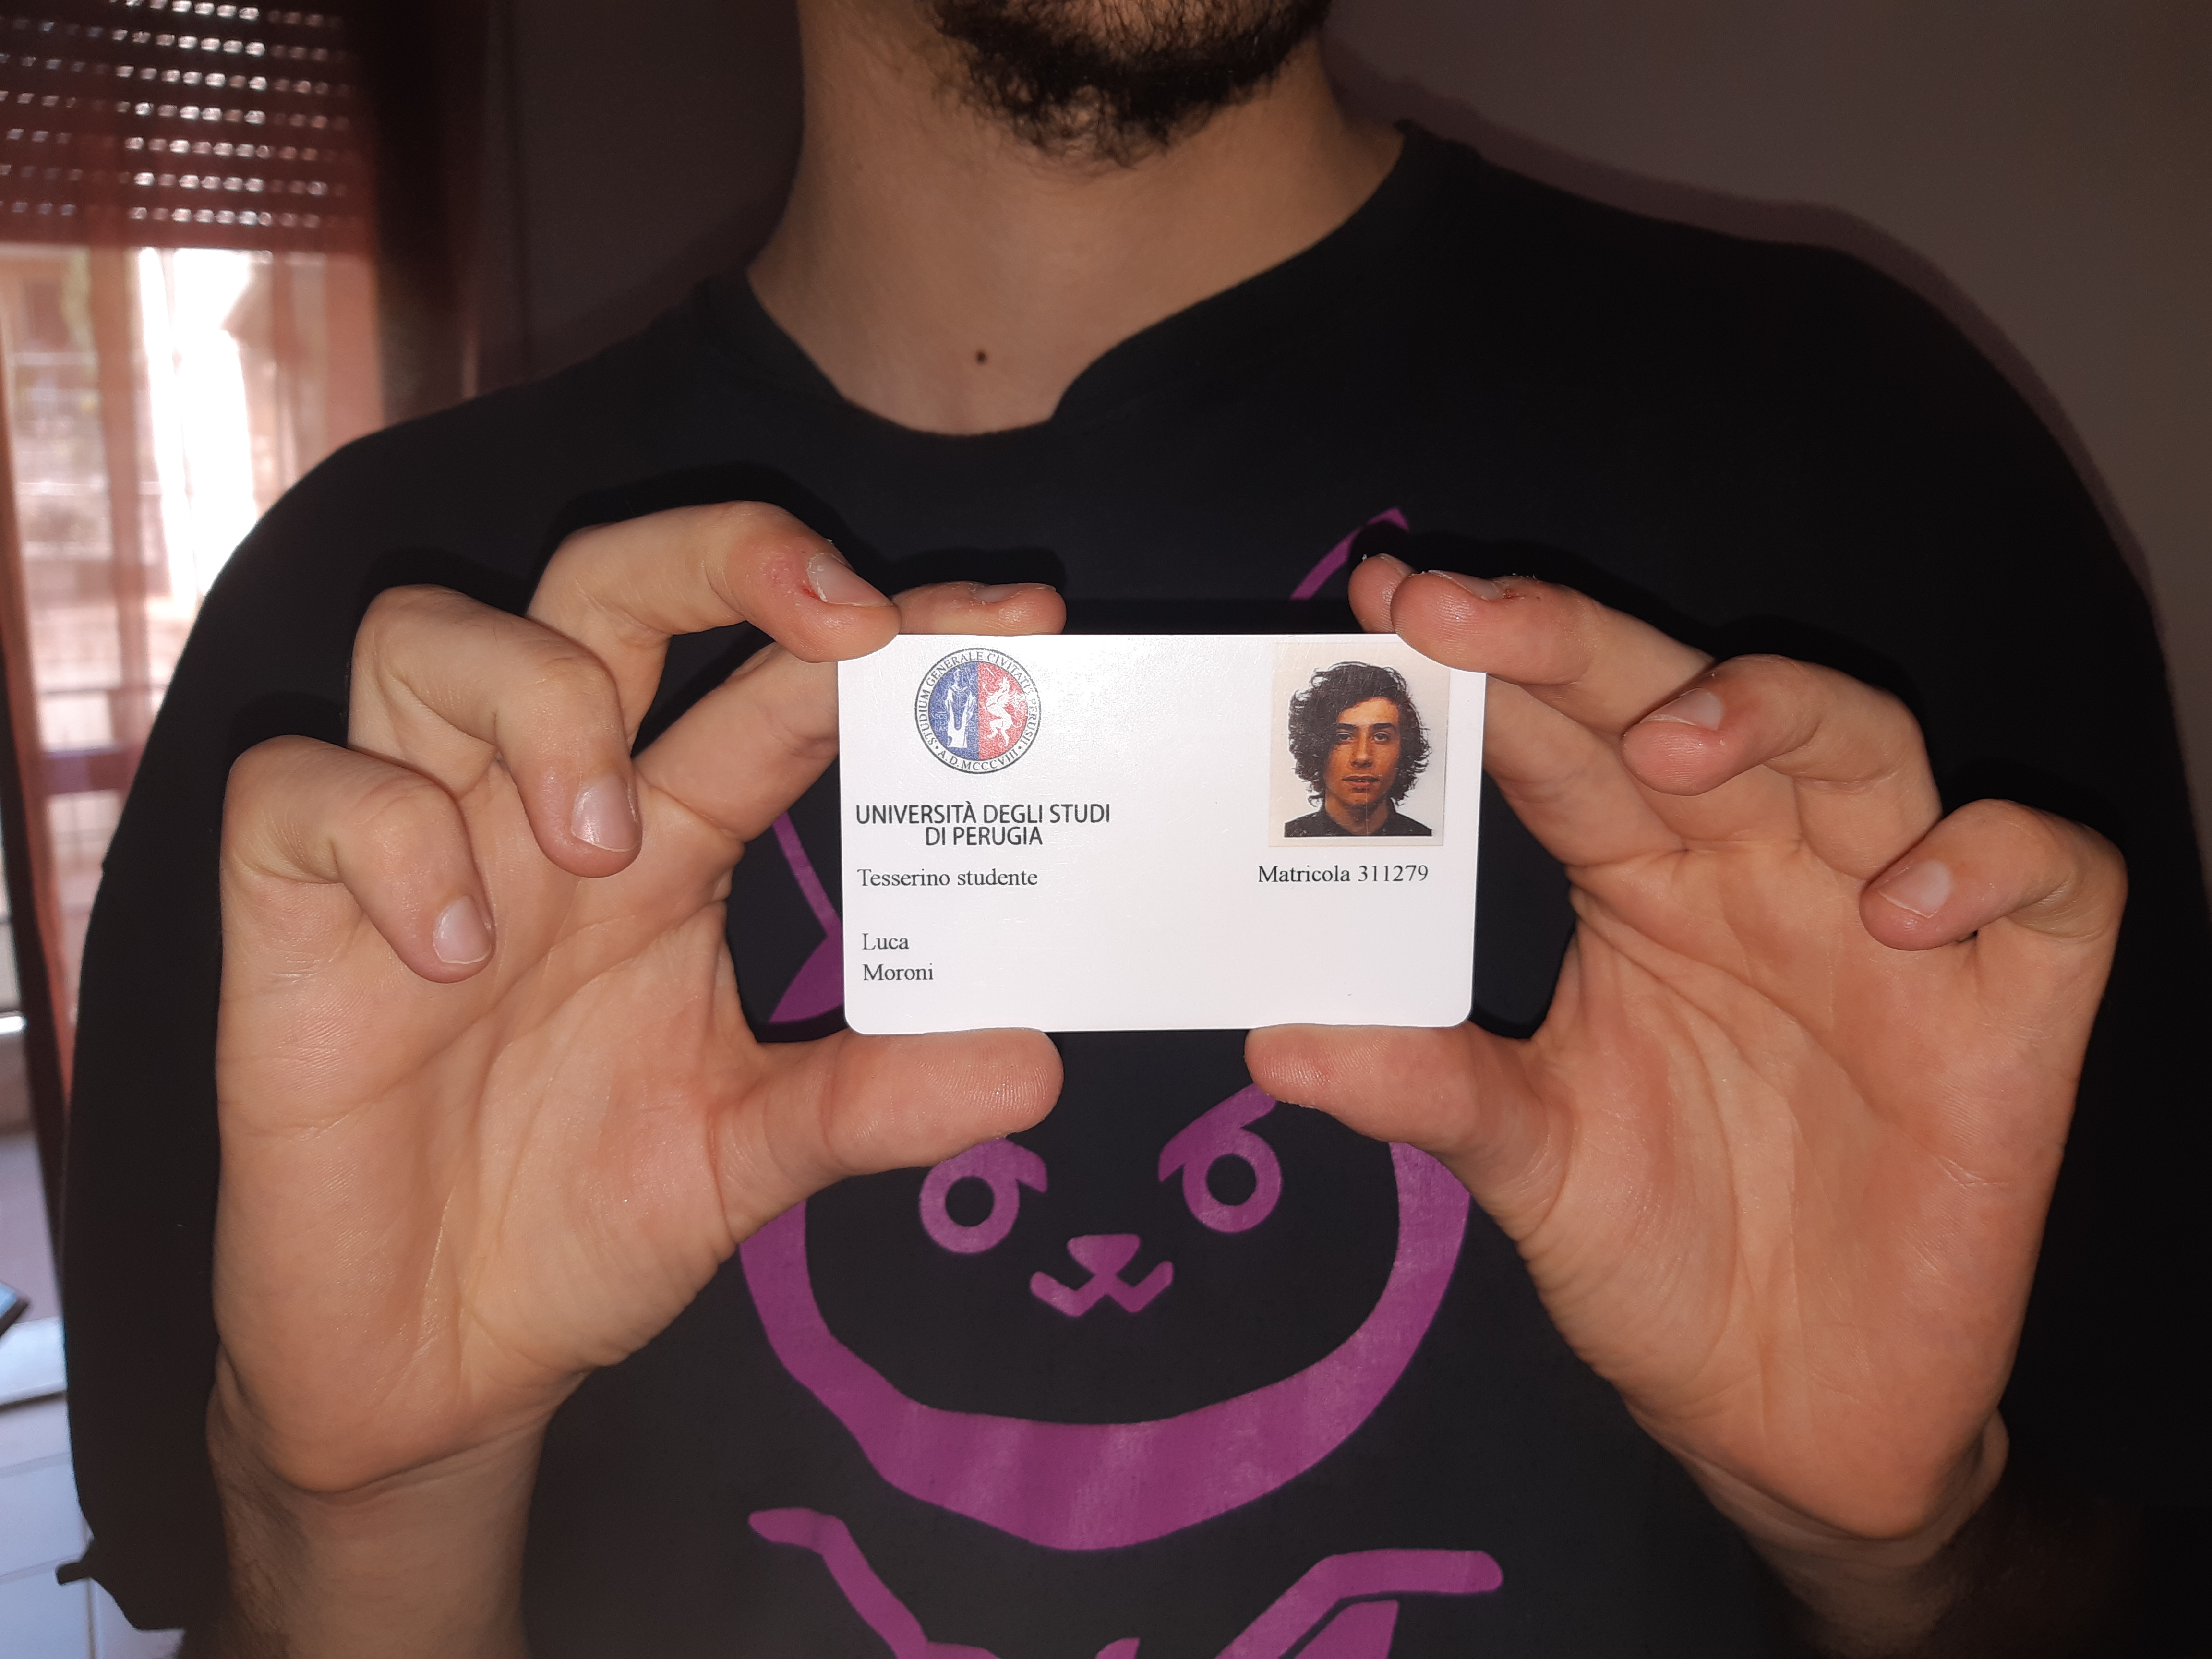
\includegraphics[width=\textwidth,height=\textheight,keepaspectratio]{../test/test_tesserino.jpg}
\end{figure}

Output:
\inputminted{json}{../test/test_tesserino.jpg}

\begin{figure}[H]
    \caption{Caso di test PATENTE}
    \centering
    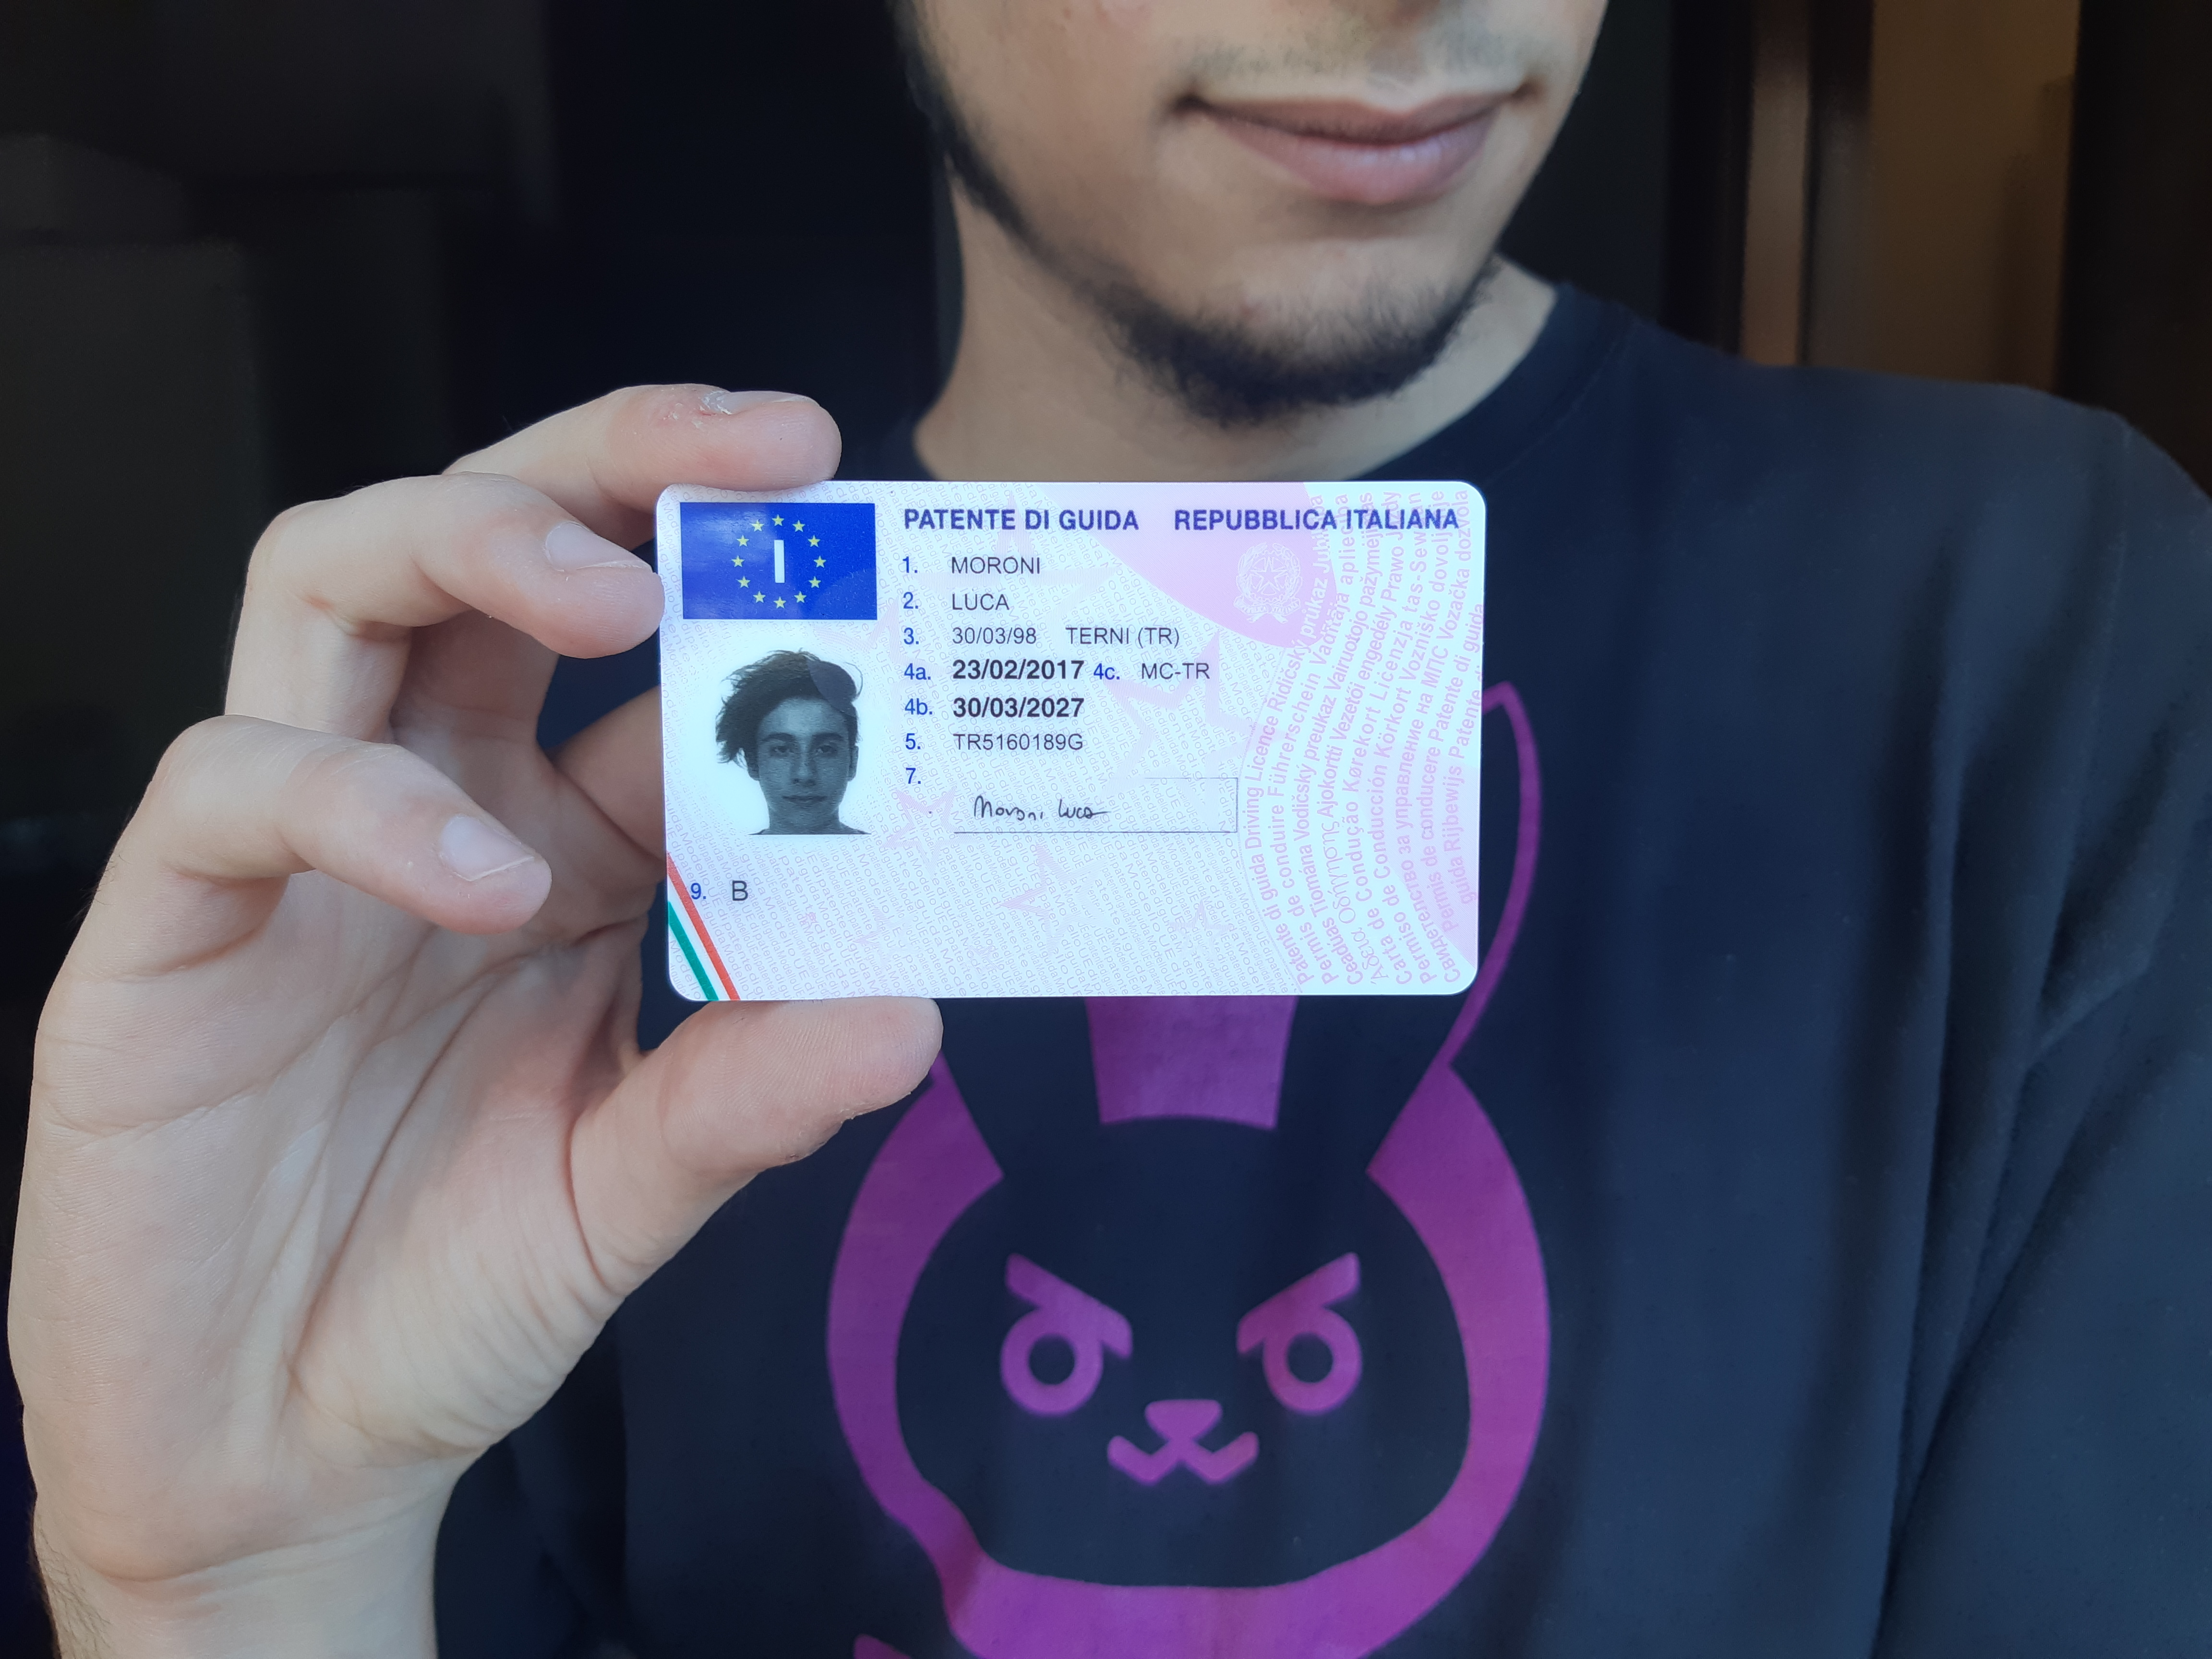
\includegraphics[width=\textwidth,height=\textheight,keepaspectratio]{../test/test_patente.jpg}
\end{figure}

Output:
\inputminted{json}{../test/test_patente.json}

\begin{figure}[H]
    \caption{Caso di test BG}
    \centering
    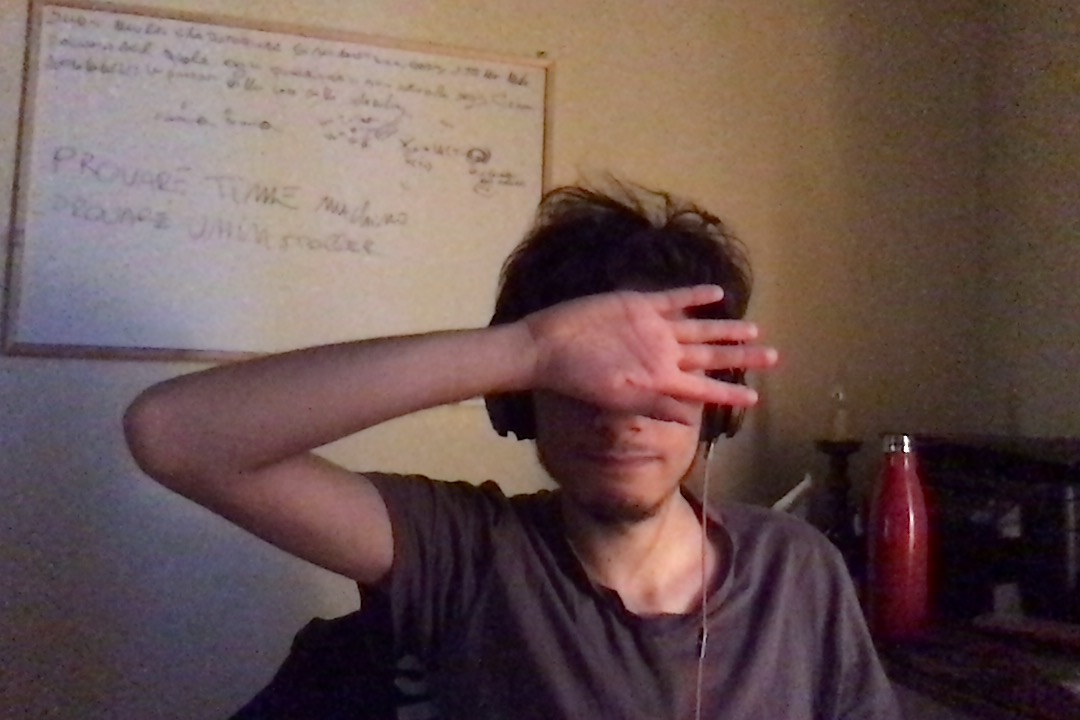
\includegraphics[width=\textwidth,height=\textheight,keepaspectratio]{../test/test_background.jpg}
\end{figure}

Output:
\inputminted{json}{../test/test_background.json}
--> foto e output

\pagebreak

\section{Training Notebook} % TODO spostare dove appropriato
\setminted[python]{
    linenos,
    breaklines,
    breakbefore=/,
    breakafter=(,
    frame=single,
    framesep=2mm
}
\setminted[text]{
    breaklines,
    breakbefore=/,
    breakafter=(,
    frame=single,
    framesep=2mm
}

Segue una copia commentata di un notebook jupyter che è stato utilizzato
per eseguire il training del dataset di esempio in Google Colab. Per
l'ultima versione dell'originale consultare la repo git.

\subsection{Preparazione dei prerequisiti}

Configuriamo la versione per le librerie utilizzate che ne richiedono
una in particolare.

\begin{minted}{python}
print("DOCUMENT RECOGNITION Training")
%tensorflow_version 1.x
!pip install keras==2.0.8
\end{minted}

Cloniamo la repo git di \mrcnn\ e la installiamo, dopodiché proseguiamo
il lavoro nella directory della repo stessa.

\begin{minted}{python}
# setup the library and its dependencies
!git clone https://github.com/matterport/Mask_RCNN.git
%cd Mask_RCNN
!python setup.py install
!pip install -r requirements.txt
\end{minted}

Montiamo la cartella Google Drive nella quale il dataset è stato
preventivamente caricato.

\begin{minted}{python}
from google.colab import drive
drive.mount('/content/drive')
\end{minted}

Scarichiamo un file di pesi preallenato su Microsoft COCO, un dataset
pensato per il riconoscimento di oggetti in contesti non isolati sul
quale faremo transfer learning per le nostre classi di documenti.

\begin{minted}{python}
!wget https://github.com/matterport/Mask_RCNN/releases/download/v2.0/mask_rcnn_coco.h5
\end{minted}

\subsection{Inizializzazione}

Importiamo le librerie e prepariamo i percorsi.

\begin{minted}{python}
import os
import sys
import json
import datetime
import numpy as np
import skimage.draw
import cv2
from mrcnn.visualize import display_instances
import matplotlib.pyplot as plt

# Root directory of the project
ROOT_DIR = os.path.abspath("./")

# Import Mask RCNN
sys.path.append(ROOT_DIR)
from mrcnn.config import Config
from mrcnn import model as modellib, utils

# Path to trained weights file
COCO_WEIGHTS_PATH = os.path.join(
    ROOT_DIR, "mask_rcnn_coco.h5")
\end{minted}

Definiamo la nostra configurazione di \mrcnn\ derivando la classe
\texttt{Config}.

\begin{minted}{python}
class CustomConfig(Config):
    """
    Configuration for training on the dataset provided on
    Google Drive. Derives from the base Config class and
    overrides some values.
    """
    # Give the configuration a recognizable name
    NAME = "document"

    # We use a GPU with 12GB memory, which can fit two
    # images. Adjust down if you use a smaller GPU.
    IMAGES_PER_GPU = 2

    # Number of classes (including background)
    NUM_CLASSES = 1 + 2  # Background + documents

    # Number of training steps per epoch
    STEPS_PER_EPOCH = 150

    VALIDATION_STEPS = 25

    LEARNING_RATE=0.006

    # Skip detections with < 90% confidence
    DETECTION_MIN_CONFIDENCE = 0.9
\end{minted}

CustomDataset estende la classe Dataset di \mrcnn\ per
permettere il caricamento dei dati dal particolare albero di
cartelle in cui abbiamo memorizzato il dataset.
Per ``mask'' (maschera) si intende la regione di ogni
immagine occupata dall'oggetto da riconoscere.

\begin{minted}{python}
class CustomDataset(utils.Dataset):
    def load_custom(self, dataset_dir, training=True):
        """
        Loads dataset from our directory structure. Every
        image containing directory must have inside an
        annotations file named "via_regions.json"

        Parameters:
        dataset_dir: path of the root folder of the dataset
        training: switch between training and validating
                  datasets
        """

        if training:
            dataset_dir = os.path.join(dataset_dir, "training/")
        else:
            dataset_dir = os.path.join(dataset_dir, "validating/")

        # Add classes.
        self.add_class("dataset", 1, "tesserino")
        self.add_class("dataset", 2, "patente")

        # Load annotations
        # VGG Image Annotator saves each image in the form:
        # { 'filename': '28503151_5b5b7ec140_b.jpg',
        #   'regions': {
        #       '0': {
        #           'region_attributes': {},
        #           'shape_attributes': {
        #               'all_points_x': [...],
        #               'all_points_y': [...],
        #               'name': 'polygon'}},
        #       ... more regions ...
        #   },
        #   'size': 100202
        # }
        # We mostly care about the x and y coordinates of
        # each region

        dir_list = [
            dir_
            for dir_ in os.listdir(dataset_dir)
            if os.path.isdir(os.path.join(dataset_dir, dir_))
        ]

        for dir_ in dir_list:
            iter_dir = os.path.join(dataset_dir, dir_ + "/")

            print("iterating: {0} ...".format(iter_dir))

            annotations1 = json.load(open(
                os.path.join(iter_dir, "via_regions.json")))
            # don't need the dict keys:
            annotations = list(annotations1.values())

            # The VIA tool saves images in the JSON even if
            # they don't have any annotations. Skip
            # unannotated images.
            annotations = [
                a for a in annotations if a['regions']]

            # Add images
            for a in annotations:
                # Get the x, y coordinaets of points of the
                # polygons that make up the outline of each
                # object instance. There are stores in the
                # shape_attributes (see json format above)
                polygons = [
                    (
                        r['region_attributes'],
                        r['shape_attributes']
                    )
                    for r in a['regions']
                ]

                # load_mask() needs the image size to convert
                # polygons to masks. Unfortunately, VIA
                # doesn't include it in JSON, so we must read
                # the image. This is only managable since the
                # dataset is tiny.
                image_path = os.path.join(
                    iter_dir, a['filename'])
                image = skimage.io.imread(image_path)
                height, width = image.shape[:2]

                self.add_image(
                    "dataset",
                    image_id=a['filename'],
                    path=image_path,
                    width=width, height=height,
                    polygons=polygons)

    # this method is invoked iteratively from the net during
    # training (GRADIENT DESCEND)
    def load_mask(self, image_id):
        """
        Generate instance masks for an image.

        Returns:
        masks: A bool array of shape [height, width,
               instance_count] with one mask per instance.
        class_ids: a 1D array of class IDs of the instance
                   masks.
        """

        # If not a dataset image, delegate to parent class.
        image_info = self.image_info[image_id]
        if image_info["source"] != "dataset":
            return super().load_mask(image_id)

        # Convert polygons to a bitmap mask of shape
        # [height, width, instance_count]
        info = self.image_info[image_id]
        mask = np.zeros(
            [
                info["height"],
                info["width"],
                len(info["polygons"])
            ],
            dtype=np.uint8)

        class_ids = list()
        for i, p in enumerate(info["polygons"]):
            # Get indices of pixels inside the polygon and
            # set them to 1
            rr, cc = skimage.draw.polygon(
                p[1]['all_points_y'], p[1]['all_points_x'])
            mask[rr, cc, i] = 1
            class_ids.append(
                self.class_names.index(p[0]['name']))

        # Return mask, and array of class IDs of each
        # instance. Since we have one class ID only, we
        # return an array of 1s
        return (
            mask.astype(np.bool),
            np.asarray(class_ids, dtype='int32'))

    def image_reference(self, image_id):
        """
        Return the path of the image.
        """
        info = self.image_info[image_id]
        print("reference...")
        if info["source"] == "dataset":
            print(info["path"])
            return info["path"]
        else:
            super().image_reference(image_id)
\end{minted}

Funzione di training.
Si occupa delle operazioni di carimento dei dataset di
training e validating ed esegue il trainig effuttuando tuning
di alcuni parametri.

\begin{minted}{python}
classes_ = None

def train(model):
    """Train the model."""

    global classes_

    # Training dataset.
    dataset_train = CustomDataset()
    dataset_train.load_custom(
        "/content/drive/My Drive"
        + "/Ing_sw_testing/document_dataset/",
        training=True)
    dataset_train.prepare()

    classes_ = dataset_train.class_names

    # Validation dataset
    dataset_val = CustomDataset()
    dataset_val.load_custom(
        "/content/drive/My Drive"
        + "/Ing_sw_testing/document_dataset/",
        training=False)
    dataset_val.prepare()

    # *** This training schedule is an example. ***
    # ***         Update to your needs          ***
    # Since we're using a very small dataset, and starting
    # from COCO trained weights, we don't need to train too
    # long. Also, no need to train all layers, just the
    # heads should do it.
    print("Training network heads")
    model.train(
        dataset_train,
        dataset_val,
        learning_rate=config.LEARNING_RATE,
        epochs=10,
        layers='heads')
\end{minted}

Istanziamo un oggetto di configurazione \texttt{CustomConfig}.

\begin{minted}{python}
config = CustomConfig()
config.display()
\end{minted}

Creiamo un modello in modalità training e carica i pesi MSCOCO per
effettuare il transfer learning.

\begin{minted}{python}
model = modellib.MaskRCNN(
    mode="training", config=config, model_dir="./")

weights_path = COCO_WEIGHTS_PATH

model.load_weights(
    weights_path,
    by_name=True,
    exclude=[
        "mrcnn_class_logits", "mrcnn_bbox_fc",
        "mrcnn_bbox", "mrcnn_mask"])

train(model)
\end{minted}

Salviamo i nuovi pesi ottenuti tramite transfer learning.

\begin{minted}{python}
import time
model_path = 'mask_rcnn_' + '.' + str(time.time()) + '.h5'
model.keras_model.save_weights(model_path)
print(model_path)
\end{minted}

Scarichiamo i pesi.

\begin{minted}{python}
from google.colab import files
files.download(model_path)
\end{minted}

Definiamo una nuova classe derivata da \texttt{InferenceConfig}, usata
per effettuare un piccolo test finale sulla nostra rete.

\begin{minted}{python}
class InferenceConfig(CustomConfig):
    # Set batch size to 1 since we'll be running inference on
    # one image at a time.
    # Batch size = GPU_COUNT * IMAGES_PER_GPU
    GPU_COUNT = 1
    IMAGES_PER_GPU = 1
    DETECTION_MIN_CONFIDENCE = 0.9

config = InferenceConfig()
config.display()
\end{minted}

Creiamo un modello \mrcnn\ in modalità inferenza caricando i nuovi pesi
da testare.

\begin{minted}{python}
model = modellib.MaskRCNN(
    mode="inference", config=config,  model_dir="./")

model.load_weights(model_path, by_name=True)
\end{minted}

Eseguiamo la \texttt{detection} su un'immagine non utilizzata per
allenare il modello.

\begin{minted}{python}
# Run object detection
image = skimage.io.imread(
    "/content/drive/My Drive/Ing_sw_testing"
    + "/document_dataset/testing/test2.jpg")
results = model.detect([image], verbose=1)

# Display results
r = results[0]

print(classes_)

display_instances(
    image, r['rois'], r['masks'],
    r['class_ids'], classes_, r['scores'])

print(r['rois'])
\end{minted}

\pagebreak

\textbf{Output}:

\begin{minted}{text}
Processing 1 images
image         shape: (426, 640, 3)      min:    0.00000 max:  255.00000 uint8
molded_images shape: (1, 1024, 1024, 3) min: -123.70000 max:  138.20000 float64
image_metas   shape: (1, 15)            min:    0.00000 max: 1024.00000 float64
anchors       shape: (1, 261888, 4)     min:   -0.35390 max:    1.29134 float32
['BG', 'tesserino', 'patente']
\end{minted}

\begin{figure}[H]
    \caption{Esito del Test}
    \centering
    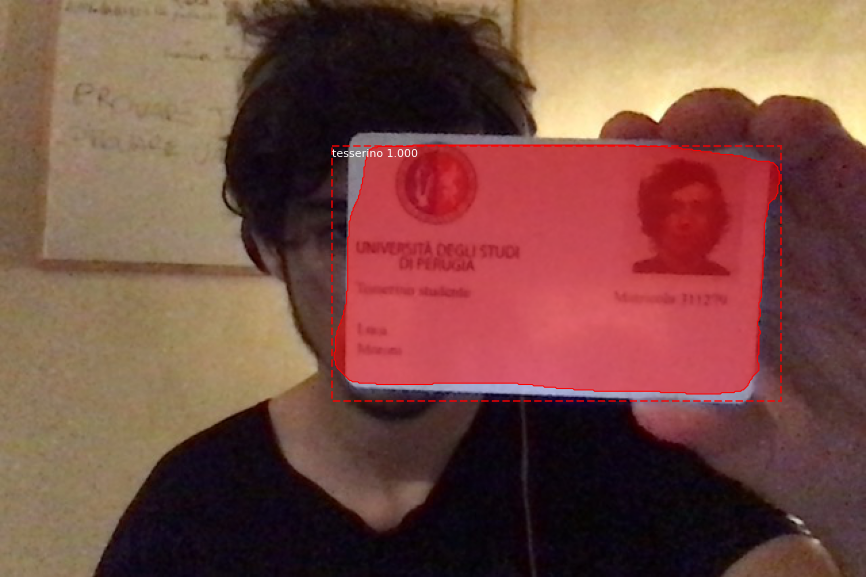
\includegraphics[width=\textwidth,height=\textheight,keepaspectratio]{document_recognition_29_1.png}
\end{figure}

\begin{minted}{text}
[[107 245 296 577]]
\end{minted}

\end{document}
